\begin{figure}[t]
% \vspace{-5pt}
\centering
 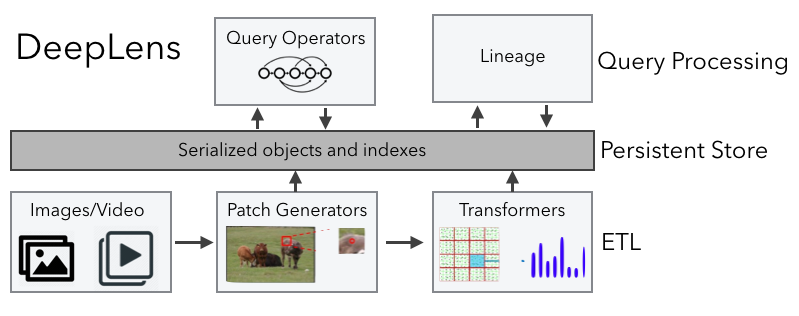
\includegraphics[width=\columnwidth]{figures/teaser.png}
 \caption{DeepLens has a dataflow-like architecture for processing visual analytics queries. All analysis is cast as relational queries on relations of image patches. Intermediate results can be materialized and indexed.  \label{teaser} }
\end{figure}

\section{DeepLens Architecture}
\textsf{DeepLens} is designed like a dataflow query processing system~\cite{graefe1994volcano}.
Figure \ref{teaser} illustrates the basic architecture with three main layers: (1) ETL, (2) Persistent Storage, and (3) Query Processing.
There are access methods which point to iterators over images derived from a filesystem or sampled from a video stream. The image dataflow is passed into a  \textbf{patch generator} that turns the image into a set of patches. Associated with each patch is a key-value dictionary storing metadata about how the patch was generated and any property of the patch. The patches are then fed into a composition of \textbf{transformers} that featurize, compress, or otherwise store detected properties of the patches into the dictionary. Over tuples of transformed patches, users can build a directed computation graph with \textbf{operators} (e.g., select, join).
Tuple-level lineage is automatically maintained by the system allowing any downstream patch to be associated with its base data.
Any of the intermediate results can be \textbf{materialized}. 
Furthermore, indexes can be built on any materialized data, either the key-value attributes or the image data.


\subsection{Visual ETL}
\label{subsection:visualETL}
In \textsf{DeepLens},  images reside in a filesystem or can be sampled from common video formats (e.g., MP4, OGG, etc.). Data are ingested into the system as 3-D dense arrays representing width and height of images, as well as  corresponding RGB channels. In a sense, this data is unstructured data. Semantics from image data have to be first extracted with computer vision algorithms before structured queries can be executed. 

\vspace{0.25em}
\noindent \textbf{Patch Generators (Extract): } As described in both examples in the previous section, we provide a library of \texttt{Patch Generators} with common primitives like object segmentation, color segmentation, and tiling. These generators take as input an iterator over raw images and return an iterator over \texttt{Patch} objects.

\vspace{0.25em}
\noindent \textbf{Transformers (Transform): } As described in the second example in the previous section, sometimes it suffices to store and process featurized representations. We provide a library of transformers with common primitives like features derived from pre-trained neural networks, image signatures, and histograms. These features can be used for matching or other types of downstream processing.

\vspace{0.25em}
\noindent \textbf{Materialize (Load): } We can load transformed data into a persistent storage which allows us to query the results of the pipeline.

\subsection{Persistent Storage}
The persistent storage is implemented with BerkeleyDB\footnote{Implemented with bsddb3 (Python binding for BerkeleyDB)}. The image and feature data is serialized in a binary format before insertion. By default, the \texttt{Patches} are stored in a sorted file by record number (or frame number for videos). This is because many queries of interest examine particular time segments of videos.
The sorted file allows for quick retrieval of temporal predicates.

\vspace{0.25em}
\noindent \textbf{Disk-Based Indexes: } We also support the construction of persistent indexes. For metadata, both hash tables and B+ trees are supported over any key (both of which are implemented with BerkeleyDB). We support construction of multidimensional indexes over dense image features or over other image properties such as bounding box coordinates (implemented with \texttt{libspatialindex}\footnote{https://libspatialindex.github.io/}).

\subsection{Query Processing}
In our initial implementation, we implement \texttt{Select} and \texttt{Join} operators. The design of the \texttt{Join} operators are the most interesting so we highlight it here. There are four physical join operators that we implement.   

\vspace{0.25em}
\noindent \textbf{Nested Loop Join: } This operator acts like a standard nested loop join operator and compares all pairs of patches from two collections and returns those that satisfy a predicate.

\vspace{0.25em}
\noindent \textbf{Metadata Index Join: } For predicates that only query the metadata in two patches, leverage an eligible index if one exists. 

\vspace{0.25em}
\noindent \textbf{Image R-Tree Join: } For predicates that compare images between patches, leverage an eligible R-tree index if one exists. 

\vspace{0.25em}
\noindent \textbf{Image Memory Join: } If one of the collections of patches can fit in memory, build an in-memory Ball-Tree. Then, probe using the other collection of patches.

\subsection{Lineage}
Many visual analytics tasks of interest relate processed results back to the base data.
For example, we might process a single set of images in two different ways, e.g., segmenting the image with an object detector and using a depth prediction model to determine relative distance between pixels.
To relate these two results we need to be able to execute queries similar to those in lineage systems~\cite{psallidas2018smoke}. 
\textsf{DeepLens} natively tracks tuple-level lineage.
Every \texttt{Patch} object relationship to the base data from which it was derived is maintained.
For example, bounding boxes that are derived can be overlayed on the original images or video.
This information is stored as attributes in the metadata key-value dictionary so indexes and queries can be natively supported on them.
